% ===========================================================================
%  06 — Evaluation
%
%  Verified claims: C-VLM-04, C-VLM-05, C-VLM-06, C-VLM-03b, C-VLM-07,
%                   C-DATA-01, C-VLM-03a, C-TRAIN-01
%  Likely claims:   C-VLM-03b, C-RUNTIME-01
%  Pilot claims:    descriptive/formative only (n=9), no inferential claims
% ===========================================================================
\chapter{Evaluation}\label{ch:evaluation}

This chapter presents empirical evidence organised around the three research
questions defined in Chapter~\ref{ch:introduction}.
Section~\ref{sec:eval-rq2} (RQ2) reports the VLM technical benchmark results
on the 13-fact ontology across three backbone models.
Section~\ref{sec:eval-rq1} (RQ1) assesses system-level technical readiness
through replay evaluation and harness regression testing.
Section~\ref{sec:eval-pilot} (RQ3) reports the formative VR pilot study with
nine participants.

Figure~\ref{fig:evaluation-dataflow} gives the chapter-level evidence map. The
three evaluation lines use different artifacts and support different kinds of
claim: benchmark metrics for RQ2, regression and replay evidence for RQ1, and
descriptive pilot data for RQ3.

\begin{figure}[htbp]
  \centering
  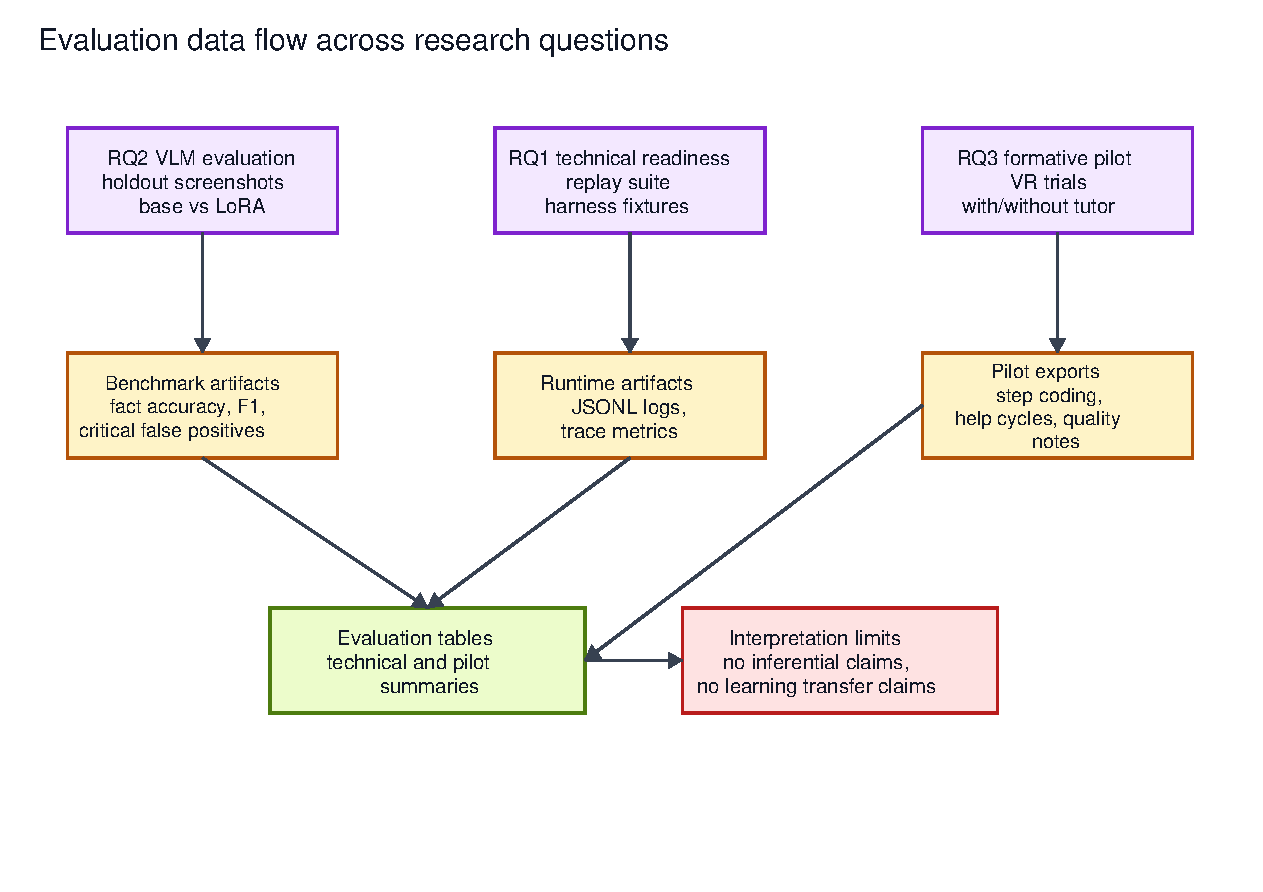
\includegraphics[width=\textwidth]{figures/fig_evaluation_dataflow.pdf}
  \caption{Evaluation and data flow across research questions. VLM benchmark
  artifacts support RQ2, replay and harness logs support RQ1 technical
  readiness, and VR pilot exports support the descriptive RQ3 findings.}
  \label{fig:evaluation-dataflow}
\end{figure}

% ===========================================================================
% --- RQ2: VLM Technical Evaluation ---
% ===========================================================================
\section{RQ2: VLM Technical Evaluation}\label{sec:eval-rq2}

The technical evaluation addresses whether a LoRA-fine-tuned VLM can reliably
extract structured visual facts from F/A-18C cockpit screenshots on holdout
data the model has never seen during training. All metrics are computed by the
automated benchmark harness described in Section~\ref{sec:method-benchmark}.

% ---------------------------------------------------------------------------
\subsection{Dataset and Training Summary}\label{sec:eval-data}

The visual fact extraction task evolved across two generations of fact
ontology. The first generation (v1) defined 8 visual facts and established the
initial training pipeline. The second generation (v2) expanded the ontology to
13 facts, aligned with the runtime contract. Table~\ref{tab:dataset-summary}
summarises the six annotated datasets.

\begin{table}[htbp]
\centering
\caption{Summary of annotated visual fact datasets.}\label{tab:dataset-summary}
\begin{tabular}{l c c c c c}
\toprule
\textbf{Dataset} & \textbf{Run} & \textbf{Facts} & \textbf{Tasks} & \textbf{Bilingual} & \textbf{Role} \\
\midrule
\texttt{vision\_sft}                     & Run-001 & 8  & 180 & yes & v1 training \\
\texttt{vision\_sft\_holdout\_run002}    & Run-002 & 8  & 50  & no  & v1 holdout \\
\texttt{vision\_sft\_holdout\_run002\_newfacts} & Run-002 & 13 & 50  & no  & v2 holdout \\
\texttt{vision\_sft\_run003}             & Run-003 & 13 & 220 & yes & v2 training source \\
\texttt{vision\_sft\_run005\_composition\_rebalance} & Run-005 & 13 & 122 & yes & v2 rebalance \\
\texttt{vision\_sft\_holdout\_run004\_random} & Run-004 & 13 & 100 & no  & v2 holdout \\
\bottomrule
\end{tabular}
\end{table}

The v2 training recipe combines Run-003 (220 reviewed tasks) with Run-005
(122 reviewed tasks, collected to rebalance under-represented fact states),
with Run-005 applied twice (Run-005$\times$2). Bilingual export (EN + ZH)
yields a combined training set of \textbf{928 rows}. The holdout sets---Run-002
newfacts (50 samples) and Run-004 random (100 samples)---are English-only with
verified \textbf{zero exact overlap} with training data.

% ---------------------------------------------------------------------------
\subsection{Qwen3.5 13-Fact V2 Results}\label{sec:eval-qwen-13fact}

The primary technical result is the performance of the Qwen3.5-9B LoRA adapter
trained on Run-003 + Run-005$\times$2 (928 rows, 4 epochs, learning rate
$2{\times}10^{-4}$, LoRA $r=16$, $\alpha=16$).
Table~\ref{tab:qwen-13fact} reports results on two independent holdout sets.

\begin{table}[htbp]
\centering
\caption{13-fact v2 benchmark: Qwen3.5-9B Base vs.\ LoRA on two holdout sets.}\label{tab:qwen-13fact}
\begin{tabular}{l c c c c c c}
\toprule
& \multicolumn{3}{c}{\textbf{Run-002 newfacts (50)}} & \multicolumn{3}{c}{\textbf{Run-004 random (100)}} \\
\cmidrule(lr){2-4} \cmidrule(lr){5-7}
\textbf{Metric} & \textbf{Base} & \textbf{LoRA} & \textbf{$\Delta$} & \textbf{Base} & \textbf{LoRA} & \textbf{$\Delta$} \\
\midrule
JSON valid       & 1.0    & 1.0    & ---  & 0.96   & 1.0    & +0.04 \\
Schema valid     & 1.0    & 1.0    & ---  & 0.96   & 1.0    & +0.04 \\
Fact accuracy    & 0.8677 & \textbf{0.9908} & +0.1231 & 0.8038 & \textbf{0.9931} & +0.1892 \\
Macro $F_1$      & 0.4513 & \textbf{0.6515} & +0.2002 & 0.4393 & \textbf{0.6100} & +0.1707 \\
Seen $F_1$       & 0.5022 & \textbf{0.9648} & +0.4626 & 0.5659 & \textbf{0.9159} & +0.3500 \\
Exact match      & 0.10   & \textbf{0.88}   & +0.78  & 0.03   & \textbf{0.92}   & +0.89 \\
Critical FP      & 11     & \textbf{4}      & $-$7   & 70     & \textbf{8}      & $-$62 \\
\bottomrule
\end{tabular}
\end{table}

The LoRA adapter achieves fact accuracy of 0.9908 (Run-002) and 0.9931
(Run-004), with sample exact match rates of 0.88 and 0.92 respectively.
Critical false positives drop by 64\% (11$\rightarrow$4) on Run-002 and 89\%
(70$\rightarrow$8) on Run-004. The base model degrades markedly on the larger
Run-004 holdout (4 schema-invalid responses, 70 critical false positives
concentrated on \texttt{fcsmc\_intermediate\_result\_visible}), while the LoRA
adapter restores format reliability and suppresses indiscriminate
hallucination.

The residual critical false positives in the LoRA adapter are concentrated on
completion-type facts: \texttt{fcsmc\_final\_go\_result\_visible} (8 on
Run-004, 1 on Run-002) and \texttt{ins\_ok\_text\_visible} (2 on Run-002).

% ---------------------------------------------------------------------------
\subsection{Gemma-4 and Qwen3.6 Backbone Comparison}\label{sec:eval-backbones}

To assess whether the training recipe generalises, the identical data recipe
(Run-003 + Run-005$\times$2, 928 rows, 13-fact ontology) was applied to two
additional backbones. Table~\ref{tab:backbone-comparison} summarises the
comparison.

\begin{table}[htbp]
\centering
\caption{13-fact v2 results across three backbones (LoRA models only).}\label{tab:backbone-comparison}
\begin{tabular}{l c c c c c c}
\toprule
& \multicolumn{3}{c}{\textbf{Run-002 newfacts (50)}} & \multicolumn{3}{c}{\textbf{Run-004 random (100)}} \\
\cmidrule(lr){2-4} \cmidrule(lr){5-7}
\textbf{Metric} & \textbf{Q3.5-9B} & \textbf{Q3.6-27B} & \textbf{G-4-31B} & \textbf{Q3.5-9B} & \textbf{Q3.6-27B} & \textbf{G-4-31B} \\
\midrule
Fact accuracy    & \textbf{0.9908} & 0.9877 & 0.9492 & \textbf{0.9931} & 0.9892 & 0.9715 \\
Seen $F_1$       & \textbf{0.9648} & 0.9479 & 0.8123 & \textbf{0.9159} & 0.9147 & 0.7959 \\
Exact match      & \textbf{0.88}   & 0.86   & 0.44   & \textbf{0.92}   & 0.86   & 0.74   \\
Critical FP      & 4      & 3      & \textbf{0} & \textbf{8} & 8      & 13     \\
\bottomrule
\end{tabular}
\end{table}

Qwen3.6-27B's base model starts substantially stronger than Qwen3.5-9B (fact
accuracy 0.91 vs.\ 0.87 on Run-002) but the LoRA gain is narrower ($\Delta
= +0.077$ vs.\ +0.123), consistent with the expectation that larger models have
less adaptation headroom under small-data fine-tuning. The Qwen3.6 LoRA
adapter achieves comparable performance to Qwen3.5 on most metrics but does
not surpass the 9B line.

Gemma-4-31B achieves zero critical false positives on Run-002, reflecting a
more conservative error style, but at the cost of lower recall (seen $F_1$
0.81 vs.\ 0.96 for Qwen3.5 on Run-002) and lower sample exact match (0.44
vs.\ 0.88). This backbone-level difference in error style---conservative
(Gemma) vs.\ assertive (Qwen)---is relevant for safety-critical deployment
decisions.

Overall, Qwen3.5-9B remains the best-performing configuration on fact
accuracy, seen $F_1$, and sample exact match across both holdouts. The data
recipe transfers across all three backbones with consistent improvements over
their respective base models.

% ---------------------------------------------------------------------------
\subsection{Error Analysis}\label{sec:eval-errors}

The 13 facts can be grouped into three difficulty categories based on the Qwen
LoRA adapter's performance. \textbf{Coarse panel presence} (6 facts:
\texttt{tac\_page\_visible}, \texttt{supt\_page\_visible},
\texttt{fcs\_page\_visible}, \texttt{bit\_root\_page\_visible},
\texttt{fcsmc\_page\_visible}, \texttt{hsi\_page\_visible}): near-perfect
classification, with the single exception of two false negatives on
\texttt{tac\_page\_visible} on Run-002. \textbf{Fine-grained state indicators}
(5 facts: \texttt{fcs\_page\_x\_marks\_visible},
\texttt{fcsmc\_intermediate\_result\_visible}, \texttt{fcsmc\_in\_test\_visible},
\texttt{fcsmc\_final\_go\_result\_visible}, \texttt{hsi\_map\_layer\_visible}):
perfect on four facts; residual false positives on
\texttt{fcsmc\_final\_go\_result\_visible} (8 on Run-004).
\textbf{Small-text recognition} (2 facts:
\texttt{ins\_grnd\_alignment\_text\_visible},
\texttt{ins\_ok\_text\_visible}): strong on the alignment text (one false
positive on Run-002); 2 false positives on \texttt{ins\_ok\_text\_visible} on
Run-002.

The base model's dominant failure mode is unidirectional hallucination on rare
states: \texttt{fcsmc\_intermediate\_result\_visible} appears in only 7 of 100
Run-004 samples, yet the base model asserts it as \texttt{seen} in 60
additional samples. The LoRA adapter eliminates this class of error almost
entirely, shifting the error profile from diffuse hallucination to focused,
interpretable residual errors on completion-type facts.

% ===========================================================================
% --- RQ1: System-Level Technical Readiness ---
% ===========================================================================
\section{RQ1: System-Level Technical Readiness}\label{sec:eval-rq1}

Beyond the component-level VLM benchmarks, the repository contains evidence
of systematic validation at the system level.

\subsection{Replay Evaluation}

The replay evaluation suite at \texttt{replay\_eval/fa18c\_startup\_v04/}
defines five test cases exercising distinct scenario types: no-operation,
battery-on, battery-and-generator-off, FCS reset and BIT, and INS alignment
(see Appendix~\ref{ch:appendix}, Table~\ref{tab:replay-cases}). Each case
includes DCS-BIOS raw captures and, where applicable, per-frame sidecar files
for vision-dependent steps. All five cases produce the expected step inference
and overlay targets, confirming that the telemetry pipeline, procedure engine,
and vision path function correctly end-to-end when driven by recorded data.

\subsection{Harness Fixture Regression}

The step harness (Section~\ref{sec:design-harness}) is covered by 20
live-fixture regression entries in the coverage matrix, each replaying a
specific telemetry snapshot through the full help cycle and asserting a
specific expected outcome. The fixtures cover: correct advancement on completed
conditions, safe rejection of wrong-target proposals (e.g., PB18 repaired to
PB5 for BIT root sub-state, S10 left-engine guidance using left-click rather
than right-click semantics), prevention of VLM evidence leakage into non-visual
steps, correct handling of moving/settling controls (refuelling probe,
arresting hook), consistent interaction semantics (mouse wheel for rotary
controls), and correct repair of partially completed steps.

\subsection{Experiment Export Infrastructure}

The experiment export pipeline (Section~\ref{sec:method-pilot}) has been
exercised on nine live VR trials, producing complete artifact sets
(trial\_summary, step\_coding, help\_cycles, action\_timeline, quality\_gate)
for each. Quality gates passed for all nine trials, with configuration hashes
verified consistent across the study. This demonstrates that the
instrumentation pipeline is functional for human-subject data collection,
though the participant/session metadata schema remains incomplete (missing
questionnaire linkage fields noted in P04's quality gate warnings).

% ===========================================================================
% --- RQ3: Formative VR Pilot Study ---
% ===========================================================================
\section{RQ3: Formative VR Pilot Study}\label{sec:eval-pilot}

A small formative pilot study was conducted with nine participants to gather
descriptive evidence on how the tutoring system supports learners during the
F/A-18C cold-start procedure compared with unaided practice. The study should
be interpreted as a preliminary field trial, not a powered controlled
experiment. Methodology details are reported in
Section~\ref{sec:method-pilot}.

\subsection{Participant and Trial Overview}

Table~\ref{tab:pilot-overview} summarises each participant's condition,
completion status, step completion, observed duration, and key interaction
counts. All data are drawn from manual step coding
(\texttt{step\_coding.csv}) and trial summaries (\texttt{trial\_summary.csv}).

\begin{table}[htbp]
\centering
\caption{Participant and trial overview. Observed duration is the wall-clock
interval from first telemetry event to last; it is not a completion time
measure for incomplete trials.}\label{tab:pilot-overview}
\small
\begin{tabular}{@{}llccccccc@{}}
\toprule
\textbf{P} & \textbf{Condition} & \textbf{Completed} & \textbf{Steps} & \textbf{Dur. (s)} & \textbf{Help} & \textbf{VLM} & \textbf{Ovrl.} & \textbf{Fallbk.} \\
\midrule
P01 & without\_tutor & no & 23/33 & 2015 & 0 & 0 & 0 & 0 \\
P02 & without\_tutor & no & 27/33 & 739  & 0 & 0 & 0 & 0 \\
P03 & without\_tutor & no & 24/33 & 243  & 0 & 0 & 0 & 0 \\
P06 & without\_tutor & no & 29/33 & 269  & 0 & 0 & 0 & 0 \\
P07 & without\_tutor & no & 19/33 & 218  & 0 & 0 & 0 & 0 \\
\midrule
P04 & with\_tutor    & yes & 33/33 & 442  & 19 & 6  & 22 & 6 \\
P05 & with\_tutor    & yes & 33/33 & 317  & 7  & 2  & 6  & 2 \\
P08 & with\_tutor    & yes$^*$ & 33/33 & 332  & 7  & 5  & 10 & 4 \\
P09 & with\_tutor    & yes & 33/33 & 1033 & 44 & 10 & 44 & 9 \\
\bottomrule
\end{tabular}

$^*$P08: auto-summary reports incomplete; manual coding confirms 33/33
completed (see data-quality note below).
\end{table}

\textbf{Completion.} All four with-tutor participants completed the full
33-step procedure. None of the five without-tutor participants completed the
full procedure; they stopped after completing 19--29 steps. The most commonly
missed steps in the without-tutor condition were S18 (FCS-MC BIT page, missed
by 5/5 participants), S19 (FCS BIT final GO, missed by 5/5), and S27 (flap
switch to AUTO, missed by 5/5).

\textbf{Observed duration.} With-tutor trials ranged from 317\,s to 1033\,s
(median 387\,s). Without-tutor trials ranged from 218\,s to 2015\,s. Because
without-tutor trials ended at different procedure points when participants
could not progress, these durations cannot be compared as completion times.

\subsection{Procedural Errors}

Table~\ref{tab:pilot-errors} reports manual error counts per participant.

\begin{table}[htbp]
\centering
\caption{Manual procedural error counts per participant (from manual step
coding). OM = omission, CO = commission, OR = order error, PA = prompting/
assistance error, SV = state violation.}\label{tab:pilot-errors}
\small
\begin{tabular}{@{}llccccc@{}}
\toprule
\textbf{P} & \textbf{Condition} & \textbf{OM} & \textbf{CO} & \textbf{OR} & \textbf{PA} & \textbf{SV} \\
\midrule
P01 & without\_tutor & 8  & 0 & 1 & 0 & 1 \\
P02 & without\_tutor & 0  & 0 & 0 & 1 & 0 \\
P03 & without\_tutor & 7  & 0 & 2 & 0 & 2 \\
P06 & without\_tutor & 2  & 0 & 0 & 2 & 0 \\
P07 & without\_tutor & 11 & 0 & 0 & 0 & 0 \\
\midrule
P04 & with\_tutor    & 0  & 3 & 0 & 3 & 1 \\
P05 & with\_tutor    & 0  & 3 & 0 & 3 & 0 \\
P08 & with\_tutor    & 0  & 0 & 0 & 0 & 0 \\
P09 & with\_tutor    & 0  & 3 & 0 & 2 & 0 \\
\bottomrule
\end{tabular}
\end{table}

\textbf{Omission errors.} The without-tutor condition shows a clear omission
pattern: four of five participants recorded 7--11 OM errors (missed steps).
In contrast, the with-tutor condition recorded zero OM errors---all 33 steps
were completed by all four participants.

\textbf{Commission and prompting errors.} The with-tutor condition shows a
different error profile: CO errors (3 per participant in P04, P05, P09) and
PA errors (2--3 per participant) replace the omission errors observed in the
without-tutor condition. These are primarily assistance-coupled errors---cases
where the tutor provided guidance that was followed but did not fully align
with the procedure specification, or where the participant executed a step
correctly in substance but with minor deviation from the prescribed sequence.

\textbf{Error totals.} Without-tutor participants averaged 7.4 manual errors;
with-tutor participants averaged 4.5. However, the error categories differ
qualitatively: without-tutor errors are dominated by omissions (mean OM =
5.6), while with-tutor errors are exclusively CO and PA (mean CO = 2.3, mean
PA = 2.0).

\subsection{Tutor Interaction}

Table~\ref{tab:pilot-tutor} summarises tutor interaction metrics for the four
with-tutor trials.

\begin{table}[htbp]
\centering
\caption{Tutor interaction summary (with-tutor condition only).}\label{tab:pilot-tutor}
\small
\begin{tabular}{@{}lccccc@{}}
\toprule
\textbf{P} & \textbf{Help cycles} & \textbf{VLM calls} & \textbf{Overlay exec.} & \textbf{Overlay rej.} & \textbf{Fallback} \\
\midrule
P04 & 19 & 6  & 22 & 0 & 6 \\
P05 & 7  & 2  & 6  & 0 & 2 \\
P08 & 7  & 5  & 10 & 0 & 4 \\
P09 & 44 & 10 & 44 & 0 & 9 \\
\midrule
Total & 77 & 23 & 82 & 0 & 21 \\
\bottomrule
\end{tabular}
\end{table}

All help cycles used the model generation path (\texttt{generation\_mode =
model}); no cycles fell back to deterministic-only mode. VLM calls were issued
for vision-priority steps (S08, S15, S18) and totalled 23 across four trials.
\textbf{Overlay rejection rate was zero}: all 82 overlay actions proposed by
the tutor passed evidence-grounding, allowlist, and schema validation. The 21
fallback events (21/77 = 27\% of help cycles) occurred when the model's
proposed overlay targets were repaired by the harness---for example, when the
model proposed a target that the harness re-mapped to a more specific
sub-state target (e.g., PB18 repaired to PB5 for BIT root).

\subsection{Data-Quality Notes}

\begin{enumerate}
\item \textbf{P08 auto-summary correction.} The automated pipeline reported
P08 as incomplete (5/33 steps). Manual telemetry review confirmed all 33 steps
reached required states. The auto-pipeline failed to reconstruct completion
evidence for vision-priority steps from passive telemetry. Manual coding
overrides the auto-summary; P08 is reported as completed with 0 manual errors.

\item \textbf{P02 questionnaire exclusion.} P02's questionnaire JSON file
contains internal \texttt{participant\_id = P01}, indicating mislabelling. P02
is excluded from any workload, TLX, or confidence summary. Task metrics
(steps, errors) from \texttt{trial\_summary.csv} and
\texttt{step\_coding.csv} are used.

\item \textbf{Duration interpretation.} Without-tutor trials ended at
different procedure points when participants could not progress further.
Observed durations are reported for completeness but do not support
completion-time comparison between conditions.

\item \textbf{Non-random assignment.} Participants were assigned to conditions
based on scheduling availability, not randomisation. Prior DCS and VR
experience varied across participants (see
Appendix~\ref{ch:appendix}, Table~\ref{tab:pilot-participants}).
\end{enumerate}

\subsection{Summary of Pilot Findings}

The pilot provides three pieces of formative evidence. First, all four
tutor-condition participants completed the full 33-step procedure, whereas
none of the five without-tutor participants did, suggesting the tutor enables
procedural progression for these participants under these conditions. Second,
the tutor condition eliminated omission errors in the coded data, but did not
eliminate all errors: assistance-coupled CO and PA errors appeared in three of
four with-tutor trials. Third, the tutoring infrastructure---telemetry
grounding, overlay dispatch, evidence validation---operated without overlay
rejections across 77 help cycles, supporting the technical feasibility of
evidence-grounded tutoring in a live VR setting.

These findings are descriptive and formative. They do not establish that the
tutor improves learning, reduces workload, or accelerates skill acquisition
relative to alternative methods. The pilot's small sample ($n=9$),
non-random assignment, and variable participant experience preclude
inferential conclusions. Larger controlled evaluation addressing these
limitations is required.
